%%%%%%%%%%%%%%%%%%%%%% 1st update for ieeeconf.cls from here %%%%%%%%%%%%%%%%%%%%%%%%%%%%%%%

%\documentclass[conference]{IEEEtran}
%\IEEEoverridecommandlockouts
% The preceding line is only needed to identify funding in the first footnote. If that is unneeded, please comment it out.
%Template version as of 6/27/2024

\documentclass[letterpaper, 10 pt, conference]{ieeeconf}  % Comment this line out if you need a4paper

%\documentclass[a4paper, 10pt, conference]{ieeeconf}      % Use this line for a4 paper

\IEEEoverridecommandlockouts                              % This command is only needed if 
                                                          % you want to use the \thanks command

\overrideIEEEmargins                                      % Needed to meet printer requirements.

%%%%%%%%%%%%%%%%%%%%%% 1st update for ieeeconf.cls until here %%%%%%%%%%%%%%%%%%%%%%%%%%%%%%%


\usepackage{cite}
\usepackage{amsmath,amssymb,amsfonts}
\usepackage{algorithmic}
\usepackage{graphicx}
% \usepackage{fontspec}
\usepackage{textcomp}
\usepackage{xcolor}
\usepackage{array}
\usepackage{makecell}
\usepackage{multirow}
\usepackage{threeparttable}
\usepackage{wrapfig}
\usepackage{hyperref}
\usepackage{subcaption}
\usepackage[T1]{fontenc}
\usepackage{lmodern}
\def\BibTeX{{\rm B\kern-.05em{\sc i\kern-.025em b}\kern-.08em
    T\kern-.1667em\lower.7ex\hbox{E}\kern-.125emX}}

\newcommand{\Comment}[1]{\textcolor{blue}{#1}}
%\newcommand{\Todo}[1]{\textcolor{red}{[TODO] #1}}
%\newcommand{\Todo}[1]{}
\newcommand{\Review}[1]{\textcolor{black}{#1}}
\newcommand{\Ishii}[1]{\textcolor{black}{#1}}

\newcommand{\Impl}[1]{\textsc{#1}}

\AtBeginDocument{
  \clearpage
  \onecolumn 
  \thispagestyle{empty}
  \vspace*{0pt} 

  \noindent
  {\LARGE IEEE Copyright Notice}

  \vspace{2em}

  \noindent
  Copyright (c) 2025 IEEE.

  \bigskip

  \noindent
  Personal use of this material is permitted. Permission from IEEE must be obtained for all other uses, in any current or future media, including reprinting/republishing this material for advertising or promotional purposes, creating new collective works, for resale or redistribution to servers or lists, or reuse of any copyrighted component of this work in other works.

  \vspace{3em}

  \noindent
  Accepted to be published in the 36th IEEE Intelligent Vehicles Symposium (IV), 2025.

  \vspace*{\fill}
  \twocolumn 
  \newpage
}


\begin{document}

%%%%%%%%%%%%%%%%%%%%%% 2nd update for ieeeconf.cls from here %%%%%%%%%%%%%%%%%%%%%%%%%%%%%%%

% \title{Comparison of Lightweight Methods for Vehicle Dynamics-Based Driver Drowsiness Detection}%\\
% %{\footnotesize \textsuperscript{*}Note: Sub-titles are not captured for https://ieeexplore.ieee.org  and
% %$should not be used}
% %\thanks{Identify applicable funding agency here. If none, delete this.}
% %}

% \author{
%     \IEEEauthorblockN{Yutaro Nakagama}
%     \IEEEauthorblockA{%\textit{School of Information Science} \\
%     %\textit{Japan Advanced Institute of Science and Technology}\\
%     \textit{JAIST}\\
%     Ishikawa, Japan \\
%     ynakagama@jaist.ac.jp}

%     \and
%     \IEEEauthorblockN{Daisuke Ishii}
%     \IEEEauthorblockA{\textit{JAIST}\\
%     Ishikawa, Japan \\
%     dsksh@jaist.ac.jp}

%     \and
%     \IEEEauthorblockN{Kazuki Yoshizoe}
%     \IEEEauthorblockA{%\textit{Research Institute for Information Technology} \\
%     \textit{Kyushu University}\\
%     Fukuoka, Japan\\
%     yoshizoe@cc.kyushu-u.ac.jp}
% }

\title{\LARGE \bf
Comparison of Lightweight Methods for Vehicle Dynamics-Based Driver Drowsiness Detection
}

\author{Yutaro Nakagama$^{1}$, Daisuke Ishii$^{1}$, and Kazuki Yoshizoe$^{2}$%
\thanks{\Ishii{This work was supported by JST, CREST Grant Number JPMJCR23M1, and JSPS, KAKENHI Grant Number 23K11969.}}% <-this % stops a space
\thanks{$^{1}$Yutaro Nakagama and Daisuke Ishii are with School of Information Science, Japan Advanced Institute of Science and Technology, Ishikawa, Japan. 
        {\tt\small \{ynakagama, dsksh\}@jaist.ac.jp}}%
\thanks{$^{2}$Kazuki Yoshizoe is with Research Institute for Information Technology, Kyushu University, Fukuoka, Japan.
        {\tt\small yoshizoe@cc.kyushu-u.ac.jp}}%
}
%%%%%%%%%%%%%%%%%%%%%% 2nd update for ieeeconf.cls until here %%%%%%%%%%%%%%%%%%%%%%%%%%%%%%%

\maketitle
%\vspace*{0.25in}
\begin{abstract}
Driver drowsiness detection (DDD) prevents road accidents caused by driver fatigue.
Vehicle dynamics-based DDD has been proposed as a method that is both economical and high performance.
However, there are concerns about the reliability of performance \Review{metrics} and the reproducibility of many of the existing methods.
\Review{For instance, 
some previous studies seem to have a data leakage issue among training and test datasets, and 
many do not openly provide the datasets they used.}
%
%This paper aims to develop a vehicle dynamics-based DDD method whose implementation and experimental results are transparent to related work.
\Review{To this end, this paper aims to compare the performance of representative vehicle dynamics-based DDD methods under a transparent and fair framework that uses a public dataset.}
%
We first develop a framework for extracting features from an open dataset \Review{by Aygun et al.} and performing DDD with lightweight ML models;
the framework is carefully designed to support a variety of configurations.
Second, we implement three existing representative methods and a concise \Ishii{random forest (RF)-based} method in the framework.
Finally, we report the results of experiments to verify the reproducibility and clarify the performance of DDD based on common metrics.
\Review{Among the evaluated methods, the RF-based method achieved the highest accuracy of 88\,\%.}
Our findings imply the issues inherent in DDD methods developed in a non-standard manner, and demonstrate a high performance method implemented appropriately.
\end{abstract}

%\begin{IEEEkeywords}
%    Driver Drowsiness Detection, 
%    Machine Learning,
%    Reproducibility Verification.
%\end{IEEEkeywords}

\section{Introduction}

\emph{Driver drowsiness detection (DDD)} methods (Sect.~\ref{sec:method}) are essential to improve road safety by mitigating accidents caused by driver fatigue~\cite{Milter1988}.
In DDD, whether the driver is {drowsy} or {awake} is determined by the signals collected from a running vehicle.
As summarized in the surveys~\cite{Albadawi2022,Perkins2023}, the signals to be used are broadly classified into:
i)~\emph{vehicle dynamics} signals such as steering angle, vehicle speed, and lane offset;
ii)~\emph{behavioral} signals that are visual cues of the driver such as eye movements and facial expressions; and
iii)~\emph{biological} signals such as EEG (electroencephalogram) and heart rate.
%
Vehicle dynamics-based methods are advantageous for their ability 
to leverage existing vehicle sensors, enabling cost-effective, non-intrusive, and real-time DDD.

The state-of-the-art DDD methods are realized using (supervised) \emph{machine learning (ML)} models.
Compared to other domains, lightweight ML methods such as SVM (support vector machine) and RF (random forest) are often favored due to hardware limitations.
As good performance has been reported by existing methods, e.g, the accuracy of $98.12\,\%$~\cite{Arefnezhad2019} and $91.22\,\%$~\cite{Wang2022} and the correct rate of $95\,\%$~\cite{Zhao2009}, we focus on DDD using lightweight ML models in this paper.

Despite the promising results of the existing vehicle dynamics-based methods,
there appears to be a discrepancy between the reported results and the DDD functions implemented in real vehicles;
\Review{for instance, the vehicle dynamics signals described in \cite{Zhao2009} appear to be inconsistent with real-world vehicle behavior.}
We also noticed some inconsistencies between the reported performance and the results of our \Ishii{reproduction experiment (Sect.~\ref{sec:exp1})};
\Review{for example, while a $91.22\,\%$ accuracy was reported~\cite{Wang2022}, we were only able to confirm $76\,\%$; also, while an AUC of $0.97$ was reported~\cite{Arefnezhad2019}, it was necessary to use test data to achieve a similar level of performance.}
\Ishii{To this end, we suspect that there may be flaws such as data leakage~\cite{Kapoor2023} that undermine the reliability of reported results.}
One of the reasons could be a non-standard development process that does not follow the standard ML practice.
In many papers, the measured metric and the experimental configuration are not clearly described, so it becomes doubtful whether they are standard.
%
\Ishii{Another issue is the reproducibility of the methods;
most DDD implementations are not available due to their proprietary nature.}

\begin{table*}[t]
    \centering
    \caption{\Review{Overview of existing vehicle dynamics-based DDD methods.}}
    \label{tab_all_ddd}
    \begin{tabular}{|m{2.8cm}|m{3.0cm}|>{\centering\arraybackslash}m{4.7cm}|>{\centering\arraybackslash}m{2.0cm}|>{\centering\arraybackslash}m{3cm}|}
        \hline
        \centering \textbf{Citation} 
        & \centering \textbf{Metric} & \centering \textbf{Input Signal} & \!\!\!\!\!\! \centering \textbf{Ground Truth} \!\!\!\!\!\! & \textbf{ML Method} \\
        \hline\hline
        Arefnezhad et al.
        \cite{Arefnezhad2019} (\Impl{SvmA}) & 98\,\% (accuracy) & SWA, SWR & KSS & {SVM} \\
        \hline
        Arefnezhad et al.
        \cite{Arefnezhad2020} & 96\,\% (accuracy) & SWA, SWR, yaw rate, lateral accel., lateral deviation from centerline 
        & %Video evaluation by expert 
        Manual evaluation
        & {CNN, CNN-GRU, CNN-LSTM} \\
        \hline
        Zhao et al.
        \cite{Zhao2009} (\Impl{SvmW}) & 95\,\% (correct rate) & SWA 
        & %Self-reported fatigue scores 
        Event occurrence
        & {SVM} \\
        \hline
        Xue et al.
        \cite{Xue2023} & 94\,\% (accuracy) & SWA, SWR, lateral offset , lateral\&longitude speed, lateral\&longitude accel., throttle angle, headway distance & $n$-back task 
        & {SVM, RF} \\
        \hline
        Wang et al.
        \cite{Wang2022} (\Impl{Lstm}) & 91\,\% (accuracy) & SWR, lateral/longitudinal accel., speed, lane offset 
        & %Phone use 
        Event occurrence
        %& \multicolumn{1}{m{4.7cm}|}{Bi-LSTM with Attention mechanism, LSTM, SVM, $k$-NN, AdaBoost} 
        & {Bi-LSTM, LSTM, SVM, $k$-NN, AdaBoost} 
        \\ 
        \hline
        Li et al.
        \cite{Li2017_2} & 88\,\% (accuracy) & SWA, yaw rate 
        & %Facial video expert evaluation 
        Manual evaluation
        & {BPNN} \\
        \hline
        Krajewski et al.
        \cite{Krajewski2009} & 86\,\% (recognition rate) & SWA & KSS & {SVM, $k$-NN, DT, LR} \\
        \hline
        \!\!\! Eskandarian et al.
        \cite{Eskandarian2007} \!\!\! & 86\,\% (accuracy) 
        & SWA, SWR, steering wheel phase plot & SDR, PERCLOS & {ANN} \\
        \hline
        Mcdonald et al.
        \cite{Mcdonald2014} & 79\,\% (accuracy) & SWA & ORD & {RF, DT, NN, $k$-NN, NB, SVM, BT}\\
        \hline
        Mcdonald et al.
        \cite{Mcdonald2012} & 79\,\% (accuracy) & SWA & ORD & {RF} \\
        \hline
        Li et al.
        \cite{Li2017} & 78\,\% (accuracy) & SWA 
        & %Facial expression-based expert evaluation 
        Manual evaluation
        & {DTW} \\
        \hline
        Sandberg et al.
        \cite{Sandberg2008} & 
        75\,\% (average of sencitivity and specificity)
        & Speed, lateral position, SWA, yaw rate & KSS & {FFNN} \\
        \hline
        Chai et al.
        \cite{Chai2019} & 75\,\% (accuracy) & SWA & KSS & {MOL, SVM, BPNN} \\
        \hline
        Jin et al.
        \cite{Jin2012} & 74\,\% (accuracy) & Speed, accel., SWA, throttle position, yaw angle 
        & %Cognitive distraction by talk 
        \!\!\! Event occurence \!\!\!
        & {SVM} \\
        \hline
    \end{tabular}
    \begin{flushleft}
        SWA: Steering Wheel Angle, 
        SWR: Steering Wheel Rate, 
        KSS: Karolinska Sleepiness Scale, 
        SVM: Support Vector Machine, 
        CNN: Convolutional Neural Network, 
        GRU: Gated Recurrent Unit, 
        LSTM: Long Short-Term Memory, 
        RF: Random Forest, 
        $k$-NN: $k$-Nearest Neighbors, 
        DT: Decision Tree, 
        LR: Logistic Regression, 
        BPNN: Back Propagation Neural Network, 
        FFNN: Feedforward Neural Network, 
        MOL: Multiple Output Learning, 
        SDR: Sleep Deprivation Recognition, 
        PERCLOS: Percentage of Eyelid Closure, 
        ORD: Observer Rating of Drowsiness, 
        ANN: Artificial Neural Network, 
        DTW: Dynamic Time Warping, 
        NB: Naïve Bayes, 
        BT: Boosted Trees, 
        Bi-LSTM: Bidirectional Long Short-Term Memory, 
        AdaBoost: Adaptive Boosting, 
        BN: Bayesian Network.
    \end{flushleft} 
\end{table*}

This paper addresses vehicle dynamics-based DDD methods based on lightweight ML models.
%We aim to develop a DDD method that is reproducible and its high performance is confirmed by a comparison with existing methods under a common configuration.
\Ishii{Our objective is to compare the performance of representative methods under the same conditions using a publicly available dataset.}
Our contributions are twofold:
\begin{enumerate}
\item \emph{A common framework for implementing DDD methods} (Sect.~\ref{sec:method}).
    We design a DDD framework that is parameterized by
    ML pipeline configurations,
    sets of features extracted from input signals, 
    feature selection methods, and
    ML methods.
    \Ishii{The framework assumes the use of an open dataset (Sect.~\ref{sec:dataset}).}
    %The framework assumes the use of multi-modal data acquisition platform (MMDAP) dataset by Aygun et al.~\cite{Aygun2024}.
    Based on the framework, we have implemented three existing methods~\cite{Arefnezhad2019,Zhao2009,Wang2022} and a simple RF method.
    %
\item \emph{Experimental results}.
    The first experiment was conducted to verify the reproducibility of the existing DDD methods and revealed several issues in their development (Sect.~\ref{sec:exp1}).
    The second experiment compared the performance of our method implementations under a common configuration (Sect.~\ref{sec:exp2}).
    As a result, we identified a high-performance DDD method using reliable metrics.
\end{enumerate}

%

\section{Related Work}
\label{sec:related_work}

There are numerous papers on vehicle dynamics-based DDD~\cite{Albadawi2022,Perkins2023}.
Tab.~\ref{tab_all_ddd} summarizes a part of the existing work.
Each column shows the following information:
\Ishii{The citation};
the performance metrics reported in the papers;
input signals representing the vehicle dynamics;
the source of ground-truth labels, which are used to train ML models; and
ML methods to develop DDD models.
%
In this paper, we select three methods, i.e., \cite{Arefnezhad2019,Zhao2009,Wang2022}, with relatively good performance from among these and use them as the subject of our experiment.
We only select methods that use lightweight ML models and whose ground-truth labels are contained in the dataset we will use;
for example, we do not select \cite{Arefnezhad2020} because it uses a large-scale model, and \cite{Xue2023} because labeling is difficult with the dataset.
%
The three methods~\cite{Arefnezhad2019,Zhao2009,Wang2022} will be analyzed in more detail in Sect.~\ref{sec:four_methods}.

%Tab.~\ref{tab_3_ddds} compares selected three approaches
%in terms of dataset characteristics, feature engineering, classification models, and evaluation metrics.
%% 3 DDDs
%Arefnezhad et al.~\cite{Arefnezhad2019} extracted features from steering angle data in both the time and frequency domains.
%They applied an adaptive neuro-fuzzy inference system (ANFIS) 
%to calculate the importance of each feature
%and performed wrapper-based feature selection.
%%
%Zhao et al.~\cite{Zhao2009} performed wavelet decomposition on steering angle data, 
%using it as features for classification.
%However, they assigned ground truth labels per entire experiment.
%%
%Wang et al.~\cite{Wang2022} extracted three features from five vehicle motion signals, 
%performed feature selection using a t-test,
%and applied a bidirectional LSTM with an attention mechanism.
%They defined task execution as a distraction and the periods before and after as alert states.

Several vehicle dynamics datasets have been developed.
%, e.g., 
%\cite{Romera2016, Li2022, Eichberger2022,Aygun2024}. 
%\cite{Li2022, Eichberger2022,Aygun2024}. 
\Review{These include PPB-Emo by Li et al. \cite{Li2022}, a multimodal dataset for emotion recognition in driving tasks; 
the dataset from the WACHSens project by Eichberger and Arefnezhad \cite{Eichberger2022}; 
and a dataset by Aygun et al.~\cite{Aygun2024}, 
the only open dataset that includes sufficient vehicle dynamics data and EEG data, and matches our use(Sect.~\ref{sec:dataset}).}
Other datasets have deficiencies in terms of vehicle data type, EEG data, event occurence data, recording frequency, open accessibility, etc.
%
%as they lack key aspects such as the variety of vehicle dynamic information, appropriate sampling rates, specialized tasks designed to induce driver distraction, reliable measures of driver drowsiness, and open accessibility. The publicly available dataset by Aygun et al. \cite{Aygun2024}, utilized in this study, is one of the few datasets that meets these criteria. Therefore, it is expected to serve as a valuable resource for future research in this domain.

% % open dataset
% This study aims to address the inconsistencies in experimental and evaluation methods 
% for vehicle-based DDD.
% We propose a standardized evaluation approach 
% by replicating the experiments of Scheutz et al. using their publicly available dataset./
% The dataset's characteristics are shown in Tab.~\ref{tab_aygun_data}.
% The Scheutz dataset includes vehicle dynamics data, 
% such as steering angle, lane offset, and acceleration, 
% along with physiological signals, such as EEG.
% It was collected from a driving simulation environment 
% designed to induce various cognitive states. 
% The dataset is synchronized across multiple sensors,
% making it suitable for evaluating ML models for drowsiness detection.

{The models in \cite{Arefnezhad2019,Krajewski2009,Sandberg2008,Chai2019}} are trained using the KSS (Karolinska sleepiness scale), which is a subjective evaluation metric, as the source of the ground truth. 
In contrast, we employ EEG signals, objective physiological data capable of real-time monitoring of the driver's arousal state. 
%
DDD using EEG analyzes brain activity to assess alertness in real-time~\cite{Jung1997}. 
%EEG sensors placed on the scalp measure electrical signals, where increased theta power is associated with drowsiness and higher beta activity indicates wakefulness. 
Since EEG provides a direct physiological measure of fatigue, it can detect drowsiness earlier than behavioral signs. 
ML models process EEG spectral features to classify alertness levels and trigger warnings, offering an objective approach to fatigue detection~\cite{Jap2009}.
%
%DDD can be performed using either EEG signals or vehicle behavior data, each with distinct advantages and limitations. 当たり前
However, implementing an EEG-based DDD 
%provides a direct measure of brain activity, offering high sensitivity to cognitive states but 利点はすでに上に書いてある
requires intrusive and specialized equipment; 
in addition, it is prone to external vibrations and noise caused by unrelated behaviour.
Therefore, we only used the EEG data obtained in the experimental environment as the source of the ground truth.

%In contrast, vehicle data-based DDD 
%relies on driving behavior, making it more practical for real-world applications, though it may be influenced by external factors such as road conditions. 
%
% この文，意味不明？
%This study focuses on vehicle dinamics-based DDD analysis, where EEG has been shown to achieve higher accuracy compared to vehicle data. \cite{Albadawi2022, Perkins2023} %add survey

%

\section{DDD Based on the Vehicle Dynamics Data}
\label{sec:method}

%\begin{figure}[t]
%    \centering
%    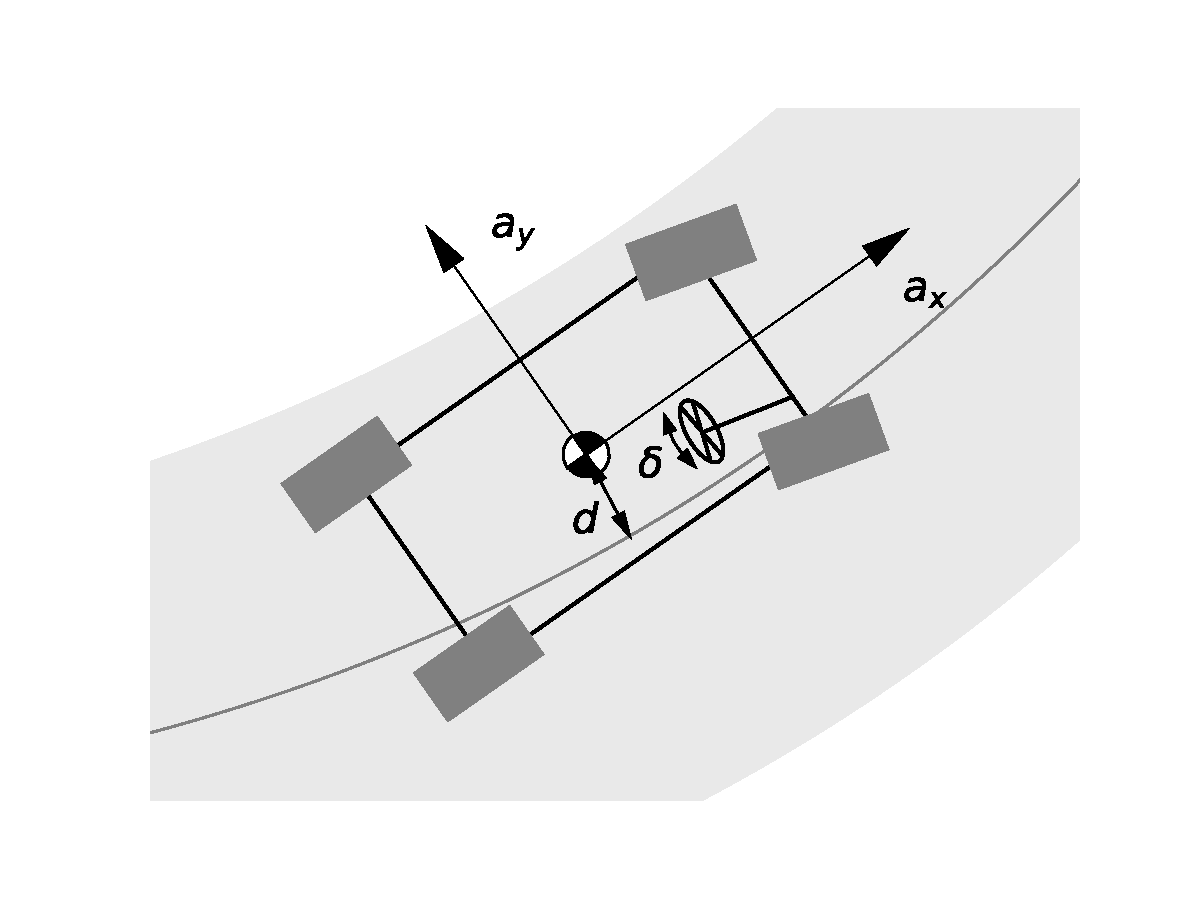
\includegraphics[width=0.3\textwidth,trim=10 70 10 80,clip]{fig/veh_dyn_new.pdf}
%    \caption{The vehicle model.}
%    \label{fig_veh_dyn}
%\end{figure}

We formulate \emph{DDD} as a binary classification problem that classifies the driver's state as either \emph{drowsy} or \emph{awake}, based on vehicle dynamics data,
which are time series data sampled from the signals of \emph{steering wheel angle (SWA)} $\theta\,\mathrm{(rad)}$, \emph{steering wheel rate (SWR)} $\dot{\theta}\,\mathrm{(rad/s)}$, \emph{lateral velocity} $v_x\,\mathrm{(m/s)}$, \emph{longitudinal} and \emph{lateral accelerations} $a_x, a_y\,\mathrm{(m/s^2)}$, and \emph{lane offset} $\delta\,\mathrm{(m)}$. 
% TODO: be sure to put spelled-out terms before.
%
\begin{wrapfigure}[10]{r}{0.28\textwidth}
\centering
    \vspace{-1em}
    \hspace*{-2.5em}
    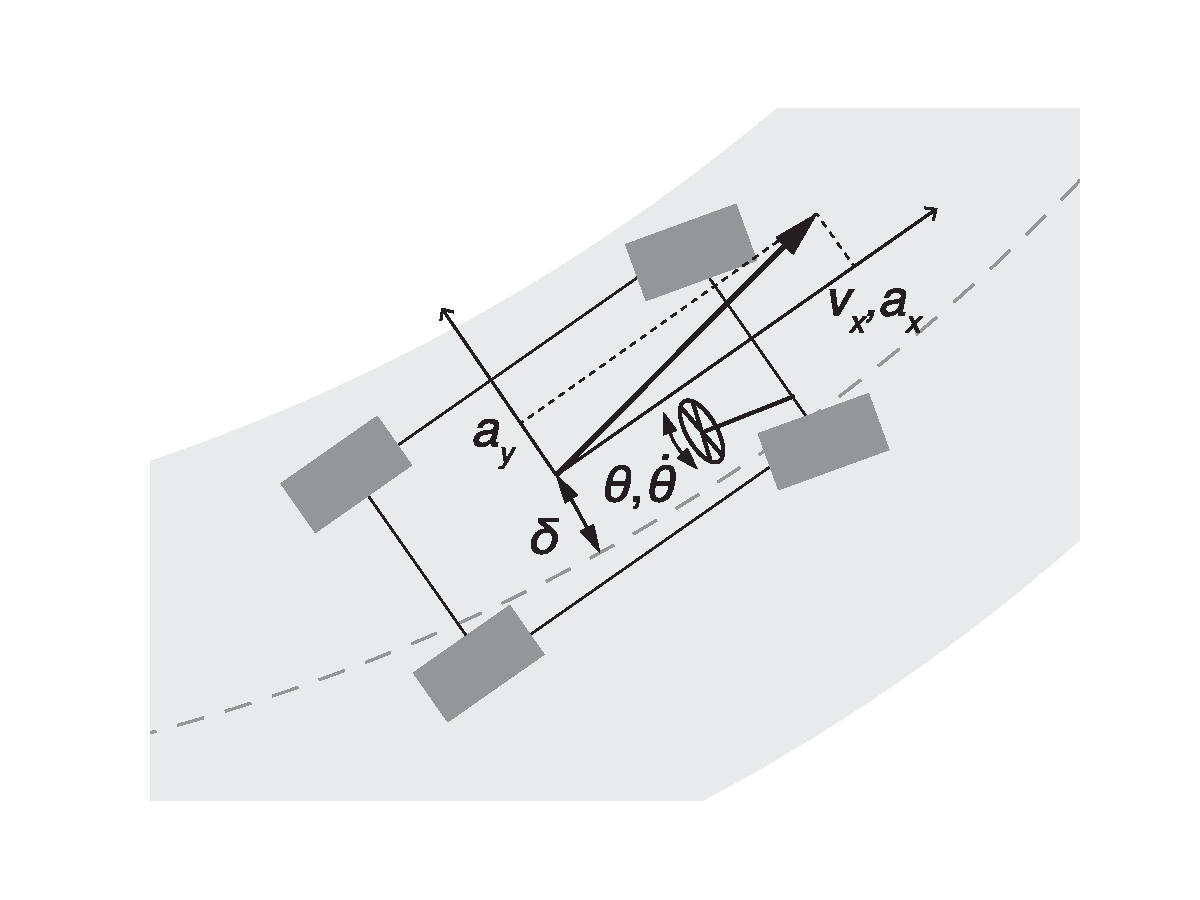
\includegraphics[width=0.35\textwidth,trim=10 70 10 80,clip]{fig/veh_dyn_mod.pdf}
    \vspace{-1em}
    \caption{The vehicle model.}
    \label{fig_veh_dyn}
\end{wrapfigure}
%
Fig.~\ref{fig_veh_dyn} illustrates the underlying vehicle model, which is basically a black box that outputs the signal data.
%
When using DDD, the data are processed as streams, but in this paper, we focus on the process of classifying the sample data from a time window independently from other time windows;
the process is parameterized by \emph{window size} and \emph{sampling frequency}.

\subsection{DDD Framework}

\Ishii{We propose a framework that extracts the common parts from lightweight DDD methods that use relatively small models based on basic ML techniques.}
An existing open dataset (Sect.~\ref{sec:dataset}) is used in common for training and evaluating the models.
We implement three methods~\cite{Arefnezhad2019,Zhao2009,Wang2022} that have  been reported to have good performance, and a basic classifier model for comparison.

\begin{figure}[t]
    \begin{minipage}[b]{.19\textheight}
   \centering
    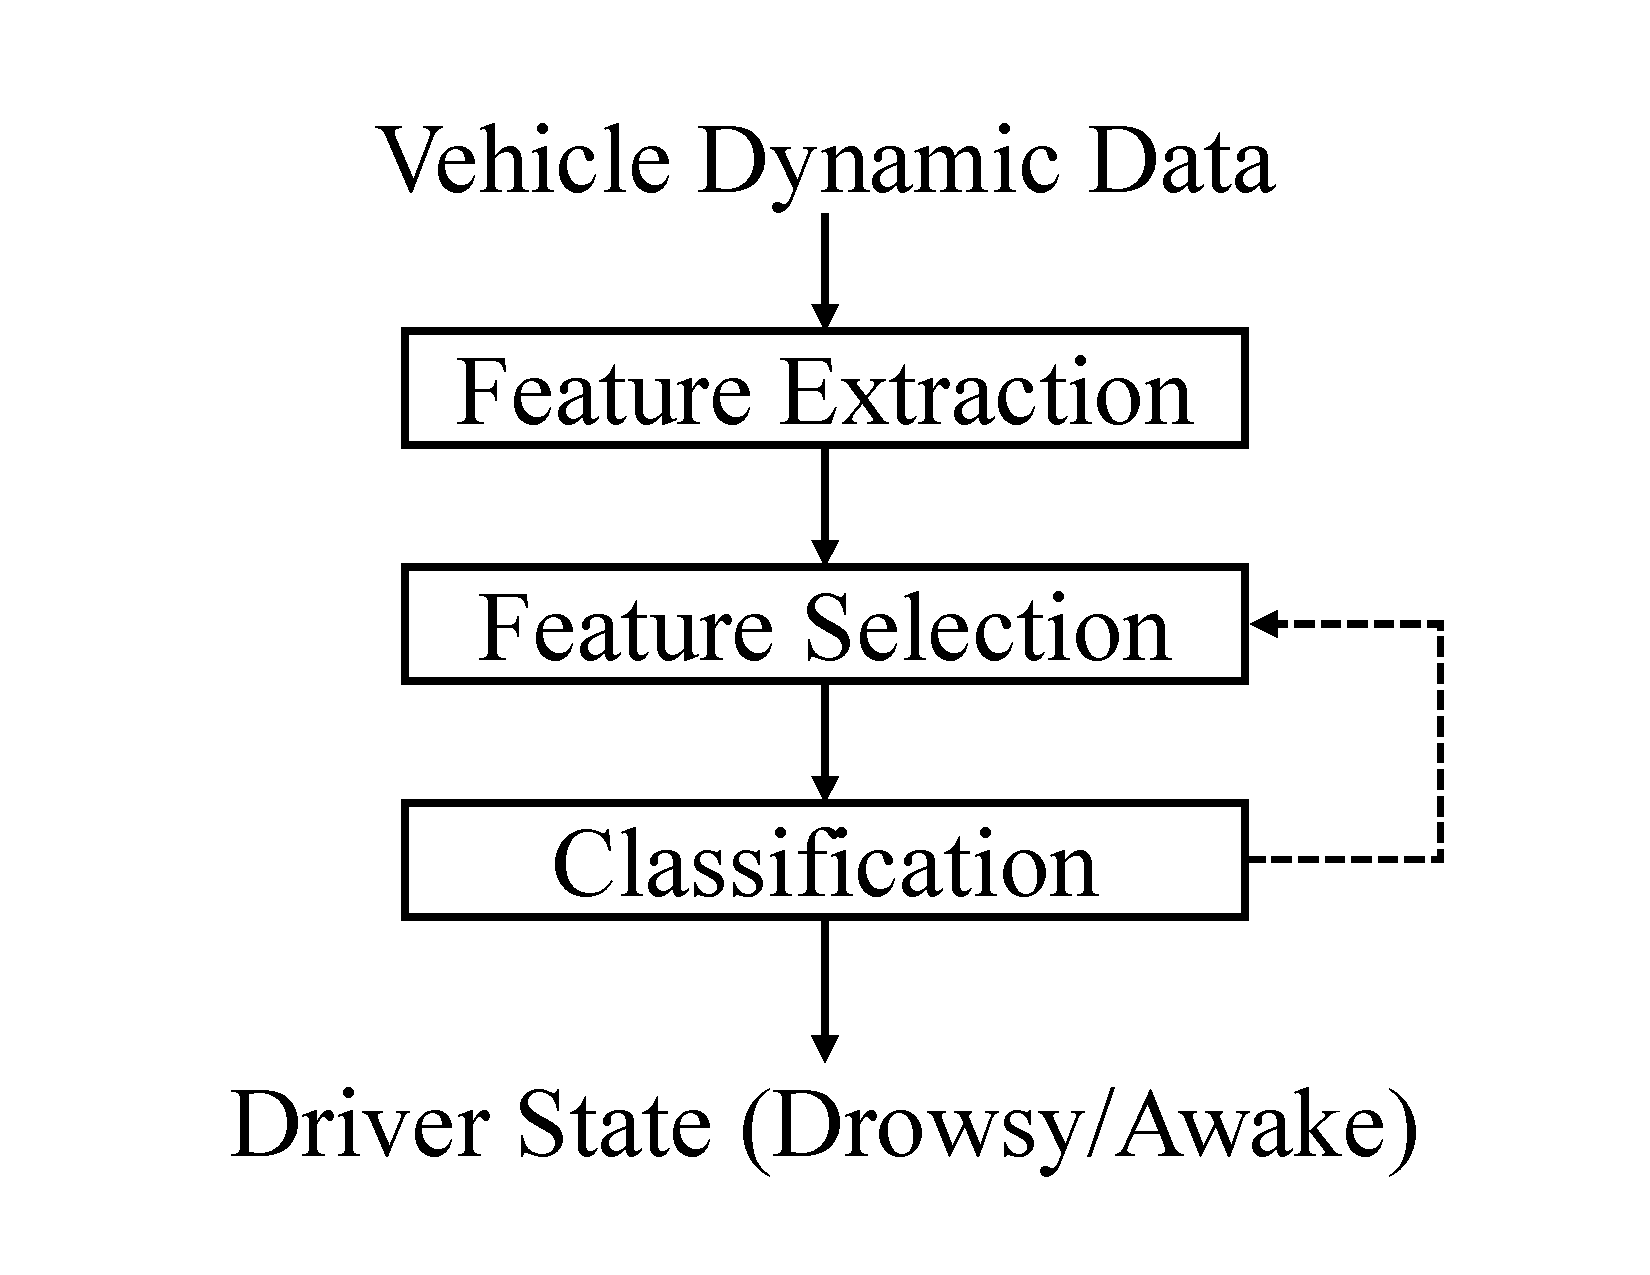
\includegraphics[width=0.8\textwidth,trim=100 50 100 50,clip]{fig/flowchart.pdf}
    \caption{DDD process.}
    \label{fig:flowchart}
    \end{minipage}
    \begin{minipage}[b]{.15\textheight}
    \centering
    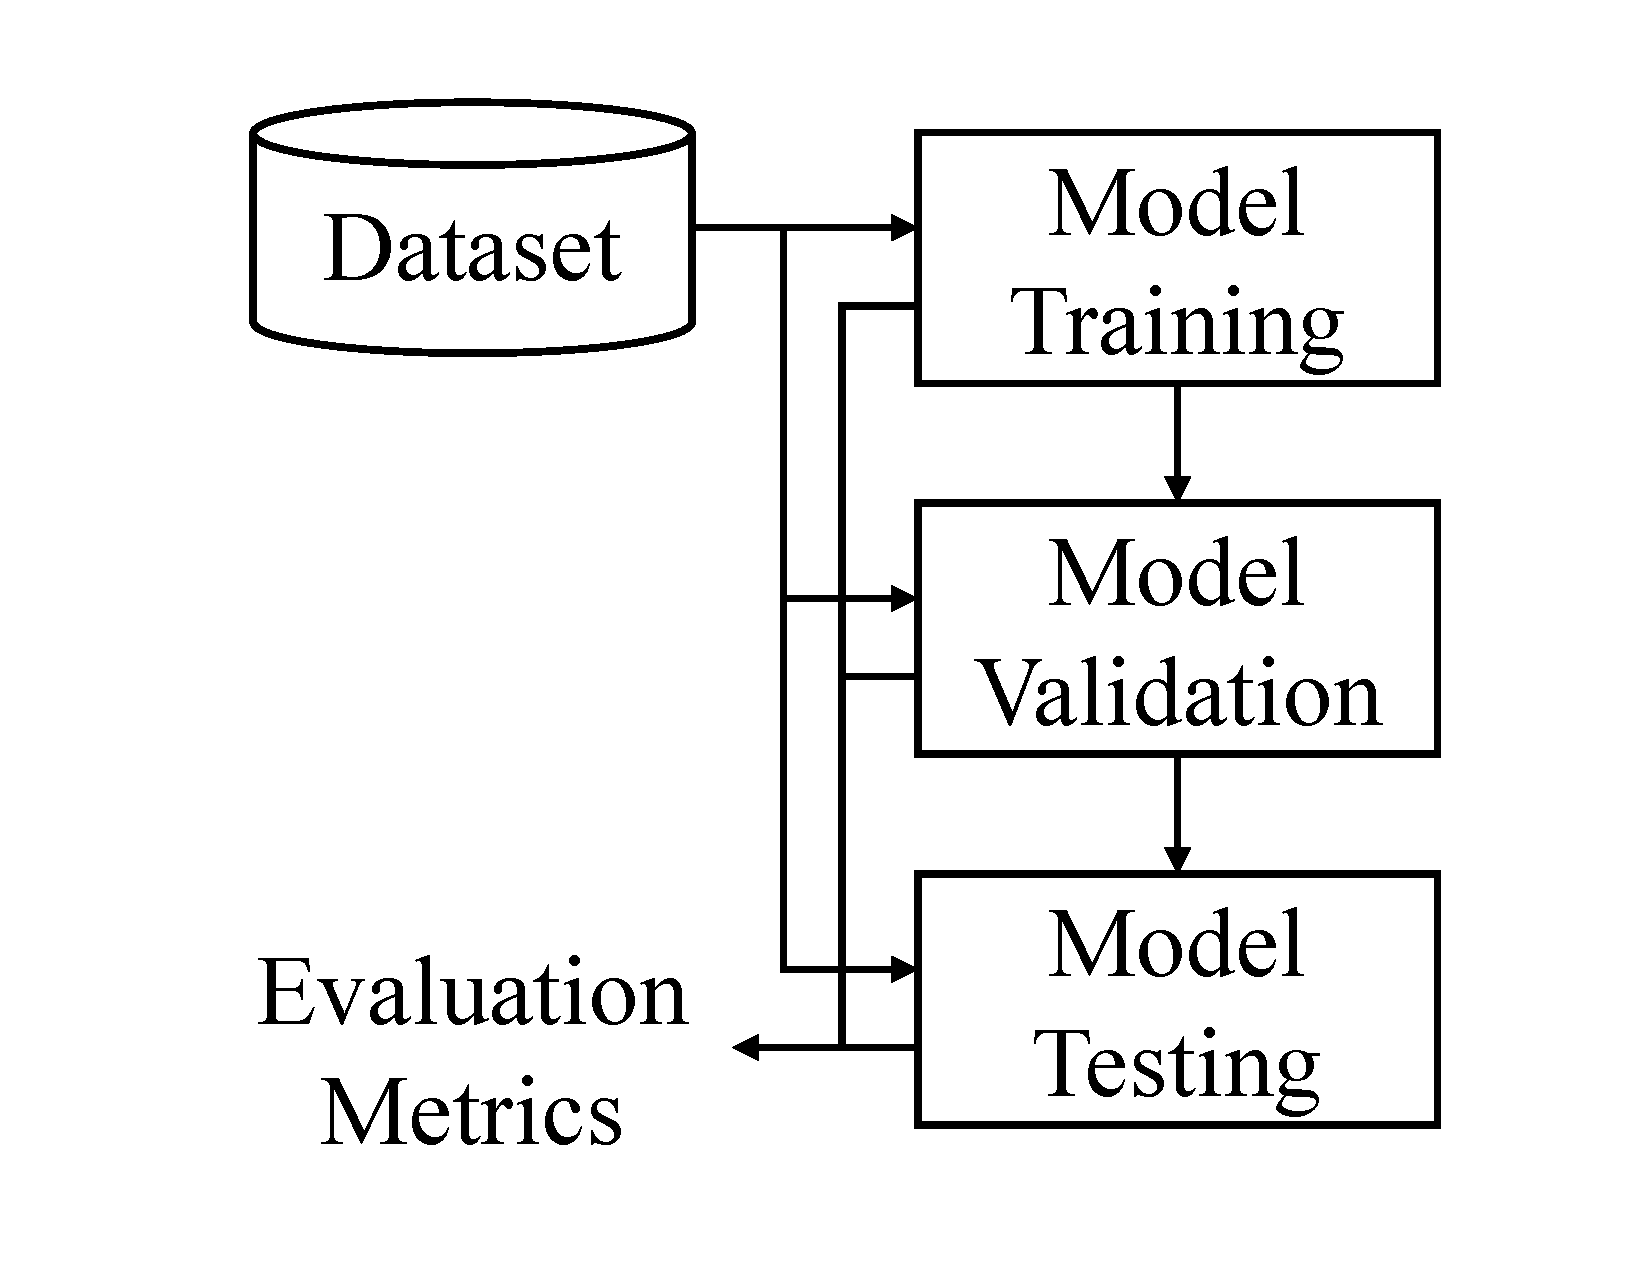
\includegraphics[width=0.9\textwidth,trim=100 0 100 0, clip]{fig/pipeline.pdf}
    \caption{ML pipeline.}
    \label{fig:pipeline}
    \end{minipage}
\end{figure}

\Ishii{The common process for the DDD methods illustrated in Fig.~\ref{fig:flowchart} is executed on the framework; it consists of the following three steps.}
\begin{enumerate}
    \item \emph{Feature Extraction}. 
    The framework computes feature values from data sampled from a time window. These include statistical values (e.g. variance and fluctuation width) and values based on wavelets. We have prepared all of the features used by the three existing methods~\cite{Zhao2009, Arefnezhad2019, Wang2022}.
    A subset of features is predefined and used for each method.
    %
    \item \emph{Feature Selection}. 
    The framework dynamically selects the likely features from a given set.
    It supports either of a standard selection method based on a statistical test or the methods used in \cite{Arefnezhad2019, Wang2022}.
    Some methods use a feedback DDD results.
    %
    \item \emph{Classification}. The resulting set of features is input to a model to obtain the driver's state.
\end{enumerate}

\subsection{ML Pipeline Configurations}
\label{sec:conf}

The development of ML models follows the \emph{pipeline} depicted in Fig.~\ref{fig:pipeline}.
The dataset is usually split for each step, i.e., training, validation and testing; however, under a \emph{data leakage configuration}, a same subset may be used among steps in a development process.
%
In our framework, we characterize various \emph{configurations} of the ML pipeline by the following three elements:
\begin{itemize}
\item \emph{Data processing method} that specifies how the dataset is split for each pipeline step and which portion to use for the evaluation;
\item \emph{Labeling} that specifies the source of the ground-truth labels (i.e. driver states) and the granularity of the data (e.g. signal fragments for a time interval) to be labeled; and
\item \emph{Hyperparameters} that specify the window size, overlap ratio, and sampling rate.
\end{itemize}

%The methods use the EEG data or the occurrence of intentional events recorded in the dataset as the ground truth during training.

\subsection{The MMDAP Dataset} \label{sec:dataset}

To implement the DDD methods, we use the \emph{multi-modal data acquisition platform (MMDAP) dataset} developed by Aygun et al.~\cite{Aygun2024,Scheutz2024}.
The dataset consists of time-series data, which record vehicle dynamics signals, road data, EEG signals and task event data required by our method;
they were collected in experiments using a driving simulator, dedicated sensors and measuring instruments.
The dataset is summarized in Tab.~\ref{tab:dataset}.

% {The road environment is a straight and four-lane highway. %simulated using a medium-fidelity driving simulator with a 180-degree field of view. 
% Traffic was light, with clear daytime conditions and a $65\,\mbox{mph}$ speed limit.
%, allowing participants to focus on experimental tasks.
%Detection response task (DRT) required participants to press a button in response to tactile stimuli delivered every 6–10 seconds via a motor on their shoulder, assessing reaction times and cognitive workload.
%Stimulus Onset Asynchrony (SOA) measured the time interval between the end of a communication task and the start of a braking event, evaluating task overlap and cognitive resource allocation.}
%
% \Todo{Process of the experiment is unclear.}
% \Todo{Experiment duration, structure of the signal data, size.}
In an experiment session described in \cite{Scheutz2024}, a participant was instructed to drive on a straight and four-lane highway.
%a vehicle simulator, where physiological monitoring devices were also attached. 
During the session, the participants were required to maintain an appropriate speed while adhering to the $65~\mathrm{mph}$ speed limit in the right lane.
%
In addition braking events and audio-based question events were systematically occured during the session.
%
The driving session included scenarios with and without the \emph{detection response task} (DRT), which required participants to press a button in response to tactile stimuli delivered every 6–10 seconds via a motor on their shoulder.
Each driving scenario covered a total distance of $37.4~\mathrm{km}$ and took approximately 25 minutes to complete. 
%At the beginning of the drive, a $5.4~\mathrm{km}$ (approximately 3 minutes) adaptation phase was included to allow participants to adjust to the driving environment. 
%Throughout the experiment, ten braking events were systematically introduced, triggered by the preceding vehicle. 
%Additionally, participants were presented with a set of 20 questions at regular intervals of approximately 30 to 60 seconds during each drive.
%
%The dataset is structured so that each subject has a separate file. 
%Within each file, time-series data are systematically organized, including vehicle dynamics data, physiological signals, and task-related details.

\begin{table}[t]
\centering
\caption{\Review{Specification of the MMDAP dataset~\cite{Aygun2024}.}}
\label{tab:dataset}
\begin{tabular}{|c|m{.31\textwidth}|} %Review
    \hline
    \multicolumn{1}{|c|}{\textbf{Category}} & \multicolumn{1}{c|}{\textbf{Description}} \\
    \hline
    \hline
    {\# Participants}
    & 82 (46\,\% female, 54\,\% male, avg. age: 20). \\
    \hline
    {Equipment} 
    & Medium fidelity partial-cab driving simulator, Enobio~8 EEG sensor system, etc.
    \\
    \hline
    {Recorded Data}
    & $a_x$, $a_y$, $v_x$, $\theta$, $\dot{\theta}$, $\delta$, DRT events, 
    brake events, 
    lane information, vehicle heading, and position. 
    ($60~\mathrm{Hz}$)
    \\
    \hline
    {EEG Data} 
    & 8~channels ($500~\mathrm{Hz}$)%. Recorded at 500Hz.
    \\
    \hline
\end{tabular}
\end{table}

% This study aims to address the inconsistencies in experimental and evaluation methods 
% for vehicle-based DDD.
% We propose a standardized evaluation approach 
% by replicating the experiments of Scheutz et al. using their publicly available dataset./
% The dataset's characteristics are shown in Tab.~\ref{tab_aygun_data}.
% The Scheutz dataset includes vehicle dynamics data, 
% such as steering angle, lane offset, and acceleration, 
% along with physiological signals, such as EEG.
% It was collected from a driving simulation environment 
% designed to induce various cognitive states. 
% The dataset is synchronized across multiple sensors,
% making it suitable for evaluating ML models for drowsiness detection.
    
%For the reproduction of Zhao et al. and Arefnezhad et al.'s methods,
In our DDD framework, we use EEG data as a source of the ground-truth labels.
%\Todo{As experimentally confirmed in \cite{}, EEG data are considered to best represent driver alertness.}
%{As confirmed in \cite{Albadawi2022, Perkins2023}, EEG data are considered to best represent driver alertness.}
{We compute frequency-specific features for the EEG signal data from multiple channels.
%from the frontal-central electrodes. 
Specifically, we analyze power spectral density in the $\vartheta$ ($4$--$8\,\mathrm{Hz}$), $\alpha$ ($8$--$13\,\mathrm{Hz}$), and $\beta$ ($13$--$20~\mathrm{Hz}$) bands~\cite{Horne2004}.
The ratio $(\vartheta+\alpha)/\beta$ is then derived to quantify drowsiness levels, based on \cite{Jap2009}. 
Following the labeling method in \cite{Arefnezhad2019}, the lower $60\,\%$ and the upper $22.2\,\%$ of the level distribution are classified as awake and drowsy, respectively.
%The intermediate range was excluded from model training to enhance the distinction between alert and drowsy states, ensuring clearer class separation for supervised learning. 
}
    
We also use DRT event occurence data for ground-truth labeling.
The binary value of either during the task or a few seconds before and after it is interpreted as drowsy and awake, respectively.

%

\subsection{DDD Methods}
\label{sec:four_methods}

\begin{table*}[t]
\centering
\caption{\Review{Details of the three DDD methods}}
\label{tab_3_ddds}
\begin{tabular}
    %{|c|m{5cm}|m{5cm}|m{4.5cm}|}
    {|c||c|c|c|}
    \hline
    \textbf{Method}
    & {\Impl{SvmA} (re-implementation of \cite{Arefnezhad2019})} 
    & {\Impl{SvmW} (re-implementation of \cite{Zhao2009})} 
    & {\Impl{Lstm} (re-implementation of \cite{Wang2022})} \\
    \hline
    \textbf{Input}
    %& $\theta$, SWR ($\dot{\theta}$) ($60\,\mathrm{Hz}$) 
    & $\theta$, $\dot{\theta}$ ($60\,\mathrm{Hz}$) 
    & $\theta$ ($25\,\mathrm{Hz}$) 
    & $\dot{\theta}$, $v_x$, $a_x$, $a_y$, $\delta$ ($10\,\mathrm{Hz}$) \\
    \hline
    {\textbf{GT Source (orig.)}}
    & KSS 
    & Self-reported fatigue scores
    & \multicolumn{1}{c|}{Event occurence} \\
    \hline
    \!\!\!\!\! {\textbf{GT Source (re-impl.)}} \!\!\!\!\!
    & EEG
    & EEG
    & \multicolumn{1}{c|}{Event occurence} \\
    \hline
    {\textbf{\# Features}}
    & 36 (sample data statistical values)
    & 8 (wavelet frequency band energy)
    & 15 (modified signal data)
    %Gaussian smoothing method, standard deviation, 2nd order Taylor approximation prediction error 
    \\ 
    \hline
    {\textbf{Selection Method}}
    & ANFIS, etc.
    %All, Fisher, t-test, correlation, mutual info, FUFES, ANFIS 
    & Not reported 
    & \multicolumn{1}{c|}{Student's $t$-test} \\
    \hline
    {\textbf{ML Method}}
    & SVM 
    & SVM 
    & Bi-LSTM with attention, etc.
    %with attention, RNN, SVM, KNN, AdaBoost 
    \\
    %\hline
    %{Evaluation metrics}
    %& 0.98 
    %& 0.95 
    %& \multicolumn{1}{c|}{0.91} \\
    \hline
\end{tabular}
\end{table*}


We consider four DDD methods, \Impl{SvmA}, \Impl{SvmW}, \Impl{Lstm}, and \Impl{RF}.
%
Based on the common DDD framework, each method is specified by an ML method and a set of features.
The first three methods aim to replicate the existing methods that have been reported to have relatively high performance; we basically use the same ML methods and feature sets as the original methods.
%
%The feature sets consist of:
%18~statistical features from time-series signals~\cite{Arefnezhad2019}; 
%8~features derived from wavelet-based analysis~\cite{Zhao2009}; and
%3~features~\cite{Wang2022}.
%
In addition, the \Impl{RF} method is prepared as an integrated method using all the feature sets.

The details of the existing methods are shown in Tab.~\ref{tab_3_ddds}.
Each row corresponds to the name of the method,
the input signal(s) to be processed (with the processing frequency indicated), 
the source of the ground-truth labels (used by the original method),
the source used by the method re-implemented in this paper,
the number of extracted features from the input signals, the feature selection method, and the ML method to generate a classification model.

\vspace{.5em}

\subsubsection{\Impl{SvmA} (\Ishii{a method using SVM and ANFIS}; re-implementation of \cite{Arefnezhad2019})}

Arefnezhad et al.~\cite{Arefnezhad2019} propose a DDD method based on the 36 statistical features computed from the values of $\theta$ and $\dot{\theta}$ in a time window.
Statistics on time (e.g. range, energy, quartiles, and Shannon entropy) and frequency (e.g. variability, spectral entropy, and average power spectral density) are used.
%across time (e.g., Range, standard deviation, energy, zero crossing rate, quartiles, Katz fractal dimension, skewness, kurtosis, sample entropy, and Shannon entropy) and frequency (e.g., Frequency variability, spectral entropy, spectral flux, center of gravity of frequency, dominant frequency, and average power spectral density.) domains.
%
The method calculates the importance of each feature using ANFIS (adaptive neuro-fuzzy inference system) and then performs a wrapper-based feature selection, which takes into account the previous classification results.
ANFIS is based on PSO (particle swarm optimization).
It uses an SMV model for the classification of the driver's states.

In the original work, ground truth labels are obtained from the KSS values surveyed for each time segment.
As mentioned previously, the re-implemented method in this paper uses labels based on the EEG in a uniform manner.

\vspace{.5em}

\subsubsection{\Impl{SvmW} (\Ishii{a method using SVM and wavelets}; re-implementation of \cite{Zhao2009})} \label{sec:ddd_svmA}

The method proposed by Zhao et al.~\cite{Zhao2009} applies wavelet decomposition on the SWA data ($\theta$).
8~features are obtained by a three-layer multiwavelet packet decomposition.
Especially Geronimo-Hardin-Massopust wavelet shows the best performance in \cite{Zhao2009}.
Among several wavelets, it has been reported that GHM (the Geronimo-Hardin-Massopust wavelet) shows the best performance;
thus, we also use GHM in our re-implementation.
%This approach effectively captures the energy distribution across distinct frequency bands, enabling a detailed representation of underlying drowsiness characteristics.
The classification model is based on SVM. 

The original implementation is based on the ground truth obtained for each entire set of experiment.
Our re-implemented method uses EEG-based labels obtained for each time window.

\vspace{.5em}

\subsubsection{\Impl{Lstm} (\Ishii{a method using LSTM}; re-implementation of \cite{Wang2022})}

Wang et al.~\cite{Wang2022} proposes an LSTM-based method for time-series DDD.
It is based on the 3~feature signals, extracted from each of 5~input signals, i.e., $\dot{\theta}$, $v_x$, $a_x$, $a_y$, and $\delta$; a total of 15~feature signals are used.
The feature signals are obtained by applying each of the statistical processes called
``mean,'' ``standard deviation,'' and ``predicted error.''
%``Mean'' represents the signal with Gaussian smoothing applied;
%``Standard Deviation (SD)'' quantifies variability and serves as an indicator of driving stability.
%``Predicted Error (PE)'' estimated using a second-order Taylor approximation,
%     reflecting the smoothness of control dynamics.
%
The method then performs feature selection using $t$-test.
The classification is done with a bidirectional LSTM with an attention mechanism.

The original experiment was based on the scenario of receiving a phone call while driving.
DDD is a classification of whether (drowsy) or not (awake) the driver is responding to the call.
Accordingly, the ground truth is based on the time periods during which the call occurs.
%
In our re-implementation, we utilize the results using DRT events in the MMDAP dataset.
As original, the ground truth is based on whether or not an event occurs.

\vspace{.5em}

\subsubsection{\Impl{RF} (\Ishii{a method using random forest})}

\Review{We propose a simple 
%but effective % かどうかは評価実験前に書かないほうがよい．
DDD method based on a classification model generated with RF~\cite{Breiman2001}.
%
This method assumes the 6 vehicle dynamics signals and uses the features extracted using all previously mentioned methods. 
%The model is trained using the six vehicle dynamics signals described in Sect.~\ref{sec:method}. % 自己参照しちゃダメ．
%Features are extracted using the techniques adopted by previous methods (e.g., time-domain statistics, frequency-domain energy, and wavelet-based features). % 前書いたことをまた書かない．
%
RF performs a certain degree of feature selection through its tree-based structure. 
To explicitly identify features with strong statistical relevance,
we additionally apply a univariate feature selection process, in which features are ranked by relevance using ANOVA F-values, 
The top-ranked features are then used to train the RF classifier. 
%
%The RF hyperparameters were tuned using Optuna to optimize performance.
The model is trained and evaluated using EEG-based ground-truth labels. 
%
%Compared to SVM-based (\Impl{SvmA} and \Impl{SvmW}) and LSTM-based (\Impl{Lstm}) methods, this RF approach emphasizes simplicity, low computational cost, and reproducibility under the proposed unified framework.
}

%\textcolor{red}{In this study, features were extracted from vehicle data based on selected previous DDD studies.  This chapter summarizes the each feature extraction approaches: eighteen statistical features from time-series signals following \cite{Arefnezhad2019}, eight features derived from wavelet-based analysis as proposed in \cite{Zhao2009}, and three additional features introduced in \cite{Wang2022}.}


\subsection{Implementation}\label{sec:impl}

We implemented the DDD framework and the four methods in \Impl{Python}~3.10.12.
SVM and RF models were implemented using \Impl{scikit-learn}~1.5.2. 
\Impl{SelectKBest} was used for the feature selection of \Impl{RF}.
The LSTM model of \Impl{Lstm} was implemented using \Impl{TensorFlow}~2.18.0 and \Impl{Keras}~3.6.0. 
PSO of \Impl{SvmA} was implemented with \Impl{pyswarm}~0.6.
%
Additionally, we performed a hyperparameter tuning using \Impl{Optuna}~4.1.0 for each model.
\Review{The implementation is publicly available at \url{https://github.com/YutaroNakagama/vehicle_based_DDD_comparison}.}
% \Todo{CUDA}.

% The experiments in the next sections were conducted on \Impl{Ubuntu}~22.04 with an Intel Core~i7-1270P CPU ($2.5\mathrm{GHz}$) with 15GB~RAM.
% \Todo{GPU}.

%\section{Experiment}\label{sec:exp}
%\subsection{Objectives}
%We have conducted two experiments to answer each of the following research questions:
%\begin{itemize}
%    \item \textbf{RQ1:} 
%        Can the performance metrics reported in previous studies be reproduced using our implementations and the Scheutz dataset?
%    \item \textbf{RQ2:} 
%        Which DDD method has the best performance?
%\end{itemize}
%

\section{Experiment to Check the Reproducibility}\label{sec:exp1}

\begin{table*}[t]
\centering
\begin{threeparttable}[b]
    \caption{\Review{Result of reproducibility verification.}}
    \label{t:reprod}
    %\begin{tabular}{|c|c||r|r|r|}
    %    \hline
    %    \multicolumn{2}{|c||}{} %& {Metric}
    %    & \multicolumn{1}{|c|}{{RV}}
    %    & \multicolumn{1}{|c|}{{C1}}
    %    & \multicolumn{1}{|c|}{{C2}} \\
    %    \hline
    %    \multirow{3}{*}{\Impl{SvmA}} & ``AUC'' & 0.97 & 0.97 & 0.53\\
    %        \cline{2-5}
    %        & ``Accuracy'' $(\%)$ & 98.12 & 97 & 65 \\
    %        \cline{2-5}
    %        %& \# Features & 5\phantom{.99} & 8 & 8 \\
    %        & ``\# Features'' & 5 & 8 & 8 \\
    %    \hline
    %    \multirow{1}{*}{\Impl{SvmW}} & ``Correct Rate (\%)'' & 95 & 57 & 51\\
    %    \hline
    %    \multirow{5}{*}{\Impl{Lstm}} & ``Accuracy'' $(\%)$ & 91.22 & 76 & 70 \\
    %        \cline{2-5}
    %        & ``Precision'' $(\%)$ & 94.59 & 76 & 84 \\
    %        \cline{2-5}
    %        & ``Recall'' $(\%)$ & 91.43 & 100 & 5 \\
    %        \cline{2-5}
    %        & ``F1 Score'' $(\%)$ & 92.924 & 86 & 10 \\
    %        \cline{2-5}
    %        & ``AUC'' $(\%)$ & 97.40 & 50 & 52 \\
    %    \hline
    %\end{tabular}
    \begin{tabular}{|l|r|r|r | r | r|r|r|r|r|}
        \hline
        \multirow{3}{*}{}
        & \multicolumn{3}{c}{\bf \Impl{SvmA}}
        & \multicolumn{1}{|c}{\bf \Impl{SvmW}}
        & \multicolumn{5}{|c|}{\bf \Impl{Lstm}} \\
        \cline{2-10}
        & \multirow{2}{4.75em}{\bf ``AUC''} 
        & \multirow{2}{4.75em}{\!\!\!\!\!\bf ``Accuracy'' ($\%$)\!\!\!\!\!} 
        & \multirow{2}{4.75em}{\bf ``\# Features''}
        & \multirow{2}{4.75em}{\!\!\!\!\!\bf ``Correct Rate'' ($\%$)\!\!\!\!\!}
        & \multirow{2}{4.75em}{\!\!\!\!\!\bf ``Accuracy'' ($\%$)\!\!\!\!\!}
        & \multirow{2}{4.75em}{\!\!\!\!\!\bf ``Precision'' ($\%$)\!\!\!\!\!} 
        & \multirow{2}{4.75em}{\bf ``Recall'' ($\%$)}
        & \multirow{2}{4.75em}{\!\!\!\!\!\bf ``F1 Score'' ($\%$)\!\!\!\!\!}
        & \multirow{2}{4.75em}{\bf ``AUC''}
        \\
        & & & & & & & & & \\
        \hline
        \hline
        RV & $0.97$ & $98.12$ & $5$ 
        & $95$ 
        & $91.22$ & $94.59$ & $91.43$ & $92.924$ & $0.9740$ \\
        \hline
        C1 & $0.97$ & $97\phantom{.12}$ & $8$ 
        & $57$ 
        & $76\phantom{.22}$ & $76\phantom{.59}$ & $100\phantom{.43}$ & $86\phantom{.924}$ & $0.50\phantom{40}$ \\
        \hline
        C2 & $0.53$ & $65\phantom{.12}$ & $8$ 
        & $51$ 
        & $70\phantom{.22}$ & $84\phantom{.59}$ & $5\phantom{.43}$ & $10\phantom{.924}$ & $0.52\phantom{40}$ \\
        \hline
    \end{tabular}
    \begin{tablenotes}
    %\begin{flushleft}
        \item RV: reported values.
        \item C1: result using a configuration similar to the original.
        \item C2: result using a common configuration.
    \end{tablenotes}
    %\end{flushleft}
    %\vspace{.5em}
\end{threeparttable}
\end{table*}

We have conducted an experiment to answer the following research question:
\emph{Can the performance metrics reported in previous studies be reproduced using our implementation and the MMDAP dataset?}

We used our implementation to reproduce the results close to the \emph{reported values (RVs)} in the literature.
In the experiment, the performance metric values obtained often differed considerably from RVs, probably because the metric or the configuration differed for details not described in the original papers.
In addition, it was often suspected that the configuration was not standard in some cases.
To this end, we checked the validity of the metric and configuration (Sect.~\ref{sec:conf}) used in each experiment by making a comparison between the two configurations:
\emph{C1}, a configuration that is supposed to be close to the original;
\emph{C2}, a common configuration to all experiments.

% Explanation on configurations removed.

In C2, we split the dataset at a $8:1:1$ ratio for training, validation, and testing.
Driver states were derived from the EEG data in each window and labeled.
%\Todo{We used the window size $X$, overlap ratio $X$, and sampling rate $X$.}
{We used the window size $3~\mathrm{seconds}$, overlap ratio $50~\mathrm{\%}$, and sampling rate $60~\mathrm{Hz}$.}

The RVs in the three papers and the results of our experiment with C1 and C2 are summarized in Tab.~\ref{t:reprod}.
%
In the following, we descibe how C1 was specified for each method and discuss the results.

\subsection{Reproducibility Verification with \Impl{SvmA}}

\subsubsection{Configuration}

We interpreted the metrics measured in \cite{Arefnezhad2019} as standard; they are AUC, accuracy, and the number of features (``\# features'') selected by the wrapper method.
\Review{Here, the ``number of features'' refers to the number of features finally selected from the full set during model training, and these selected features were used as inputs during evaluation.}

Since \cite{Arefnezhad2019} does not describe how the data are split, and the number of samples in their confusion matrix is almost 85\% of samples acquired from experiment,  
we assumed that the data had not been divided and that the \emph{training accuracy} was reported; we did the same in C1.
Labels had been derived from KSS but it was based on EEG in C1.
%\Todo{The total experiment duration was modified in C1?}
{The total experiment duration was approximately 164 hours in this study though only 20 hours and 36 minutes were utilized in \cite{Arefnezhad2019}.}
%\Todo{The sampling rate $X$, window size $X$, and overlap ratio $X$ were set.}
{The sampling rate $60~\mathrm{Hz}$, window size $3~\mathrm{s}$, and overlap ratio $50~\mathrm{\%}$ were set.}
%\Todo{Confusion matrices was used? What does it mean?}
% \textcolor{red}{From the confusion matrix in the original paper, the total number of samples used for evaluation is estimated to be 35079.
% Based on the experimental duration, sampling frequency, and labeling method, the total number of samples obtained from the experiment is estimated to be approximately 43000.
% Typically, the test set used for model evaluation constitutes 10\%–30\% of the entire dataset. However, the above estimates suggest that over 85\% of the experimental data might have been used for evaluation. 
% This raises the possibility that the dataset was not properly split or that the reported results reflect training accuracy rather than test performance.}

\subsubsection{Discussion}

The RVs and the values obtained with C1 were almost comparable. 
However, a significant discrepancy was observed between the results with C1 and C2.
This is due to that the results with C1 were training accuracy.
%
%Based on the details provided in their paper—including the total experiment duration, sampling rate, sliding window size, overlap ratio, KSS-based labeling, and confusion matrix—it is possible to estimate the number of experimental data points and the data used for evaluation. 
%
%Additionally, since the paper does not provide any description of data splitting, it is highly likely that their reported accuracy corresponds to training accuracy.
We believe the model trained under C1 was suffering from overfitting.
%\Todo{Why?}
{This is because optimizing the objective function for training accuracy often leads to overfitting on the training dataset, resulting in a loss of generalization performance.}
%
As usual, the test accuracy with C2 became lower.

\subsection{Reproducibility Verification with \Impl{SvmW}}

\subsubsection{Configuration}

In \cite{Zhao2009}, the metric ``\emph{correct rate}'' was evaluated.
%Based on the compatibility with our experimental results, we interpreted it as accuracy (the percentage of correct results).
Based on the analysis of the number of samples and that of misclassified samples reported in \cite{Zhao2009}, we interpreted it as accuracy (the percentage of correct results), which takes both the training and the test datasets into consideration.
%\begin{equation*}
%    \frac{\text{Total TP} + \text{Total TN}}{\text{Total Samples}}
%\end{equation*}
%Here, CR denotes the Correct Rate, TP represents True Positive, and TN represents True Negative.

According to \cite{Zhao2009}, the data was divided with a training-to-testing ratio of $3:7$ in C1.
%, which is not a conventional practice in standard evaluations.
For labeling, we used EEG data, although \cite{Zhao2009} used the participants' self-assessments.
The data were not processed with a sliding window, but the data for around 800~seconds was processed as a whole.
%\Todo{The sampling rate was set to ??.}
{The sampling rate was set to $60~\mathrm{Hz}$.}

\subsubsection{Discussion}

With both C1 and C2, the results were lower than RV.
%\Todo{We consider this is due to the adequacy of the source of the ground truth and evaluation methodology.}
We consider this is due to the adequacy of the source of the ground truth and evaluation methodology.
The results were worse with C2 than with C1.
We consider that it is more standard to measure using our ratio $training:validation:test=8:1:1$ for data splitting and the precision metric by test dataset for a classification problem like DDD. 

%However, there are three points to highlight regarding the evaluation methodology of the original study.
%Firstly, labels were assigned to approximately 800-second intervals per case. 
%This approach may not be appropriate for evaluating a driver monitoring system, where real-time fluctuations are a crucial consideration.
%Secondly, the data splitting method used in the original study is noteworthy. 
%According to the original paper, the data was divided with a training-to-testing ratio of 3:7, which is not a conventional practice in standard evaluations.
%Lastly, the metric used for evaluation, ``Correct Rate,'' is also unconventional. 
%From the results presented in their paper, it can be inferred that the following formula was used to calculate the Correct Rate, though it is not a standard evaluation method:
%
%When the labeling approach was adjusted to use time windows and the data was appropriately split, 
%it was confirmed that the accuracy decreased, as shown in the column for standardized evaluation metrics in the figure.

\subsection{Reproducibility Verification with \Impl{Lstm}} 

\subsubsection{Configuration}

As for \Impl{SvmA}, the metrics in \cite{Wang2022} were considered to be standard.
Precision, recall, F1 score were additionally used.
%
%\Todo{Explain how data set is split in C1}.
{A 5-fold cross-validation method was applied in C1.}
Driver states were classified according to whether or not the DRT events were occurred or not.
%\Todo{The sampling rate $X$, window size $X$, and overlap ratio $X$ were set.}
{The sampling rate $10~\mathrm{Hz}$, window size $10~\mathrm{second}$ without overlapping were set.}

\begin{figure}[t]
        \centerline{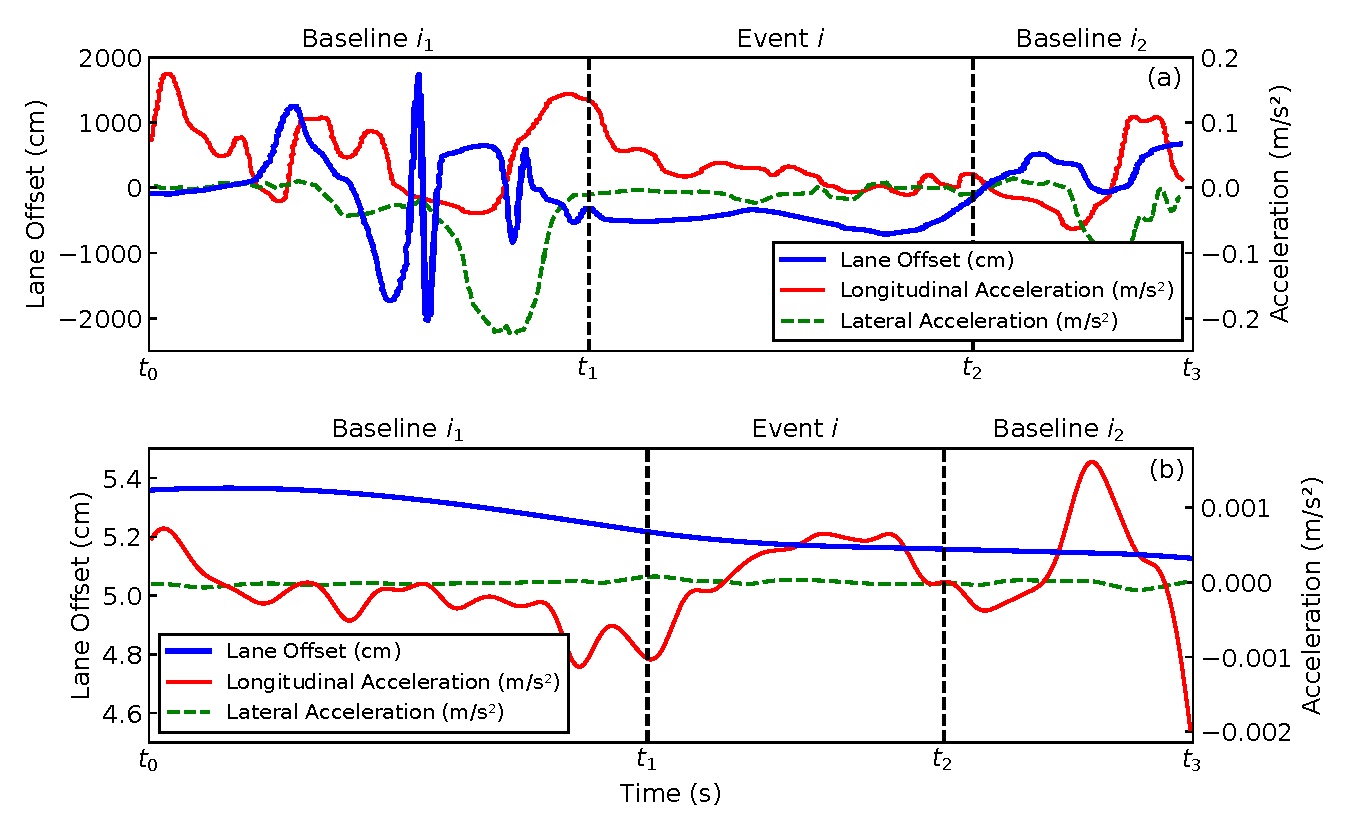
\includegraphics[width=0.5\textwidth, trim=0 5 0 0, clip]{fig/wang_sample.pdf}}
    \caption{Example input signals.}
    \label{wang_vs_ours}
\end{figure}

\subsubsection{Discussion}

The values we obtained were significantly lower than RVs.
%
Fig.~\ref{wang_vs_ours} shows both signal examples from \cite{Wang2022} and from the MMDAP dataset.
%In the first example, there seems to be a significant difference in the trend depending on whether it is the Baseline time or the Event time.
\Review{Fig.~\ref{wang_vs_ours}~(above) presents a sample from the dataset described in \cite{Wang2022}, where a clear change in signal patterns can be observed between the baseline and event intervals.} 
%In contrast, we do not see any clear trend differences in MMDAP dataset.
\Review{In contrast, Fig.~\ref{wang_vs_ours}~(below) shows an example from the MMDAP dataset, where such trend differences are not evident.} 
This may account for the gap between the results with C1 and the RVs.

{Achieving $100\,\%$ recall indicates that all positive instances are correctly identified; however, it may come at the cost of reduced precision. 
This could lead to a higher number of false positives. }
%\Todo{Explain why the C1 and C2 differed.}
{In C1, event-based labeling was conducted following the original study, 
while C2 utilized EEG data to label driver alertness levels. 
The difference in labeling approaches revealed variations in model performance, even with the same model and dataset.}
%

\subsection{Summary}

In the experiment, we were only able to reproduce the reported performance partially under the standard interpretation of the metrics.
It was shown that some results reported in the literature probably reported the performance metrics of the training step, not the test step.
The result suggests that standardization of the evaluation process will be valuable.

%

\section{Evaluation of the \Impl{RF} Method}\label{sec:exp2}

The second experiment compared the four methods to answer the question:
\Ishii{\emph{How does the performance of the \Impl{RF} method compare to the other three methods?}}

\Review{While Sect.~\ref{sec:exp1} focused on reproducing and evaluating three existing methods, this section adds the proposed \Impl{RF} method into the comparison. By evaluating all four methods under the same configuration C2 and using standard performance metrics such as accuracy and AUC, we aim to provide a fair comparison among the methods and assess the effectiveness of the \Impl{RF} method.}

\subsection{Results}

The results are shown in Tab.~\ref{tab:result_all} and Fig.~\ref{roc}.
Tab.~\ref{tab:result_all} shows the four metrics for each method.
%For the three metrics, \Impl{RF} had the best values.
Fig.~\ref{roc} illustrates the ROC curves.
%
\Review{As shown in Tab.~\ref{tab:result_all} and Fig.~\ref{roc}, \Impl{RF} achieved the best AUC (0.85) and accuracy (88\,\%) among the four methods. It also demonstrated a balanced recall (70\,\%) and reasonable precision (64\,\%), indicating both sensitivity and stability.}
%Due to the low recall score, the classification with \Impl{Lstm} will be less useful in practice.
Although \Impl{Lstm} achieved the best precision, the recall rate was relatively low.
\Review{In contrast, \Impl{Lstm} showed a recall as low as 5\%, which makes it less useful in practical applications.}

\begin{table}[t]
     \centering
     \caption{Performance comparison.}
     \label{tab:result_all}
     %\begin{tabular}{|l||c|c|c|c|c|c|}
     %     \hline
     %     %\textbf{Metric} & \textbf{RF} & \textbf{SVM\_wavelet} & \textbf{SVM\_ANFIS} & \textbf{LSTM\_DRT} \\
     %     \textbf{Method} & \Impl{RF} & \Impl{SvmA} & \Impl{SvmW} & \Impl{Lstm} \\
     %     \hline
     %     \textbf{AUC (\%)} & $\mathbf{85}$ & 53 & 49 & 52 \\
     %     \hline
     %     \textbf{Accuracy (\%)} & $\mathbf{88}$ & 65 & 49 & 70 \\
     %     \hline
     %     \textbf{Precision (\%)} & 64 & 65 & 48 & $\mathbf{84}$ \\
     %     \hline
     %     \textbf{Recall (\%)} & $\mathbf{70}$ & 65 & 49 & 5 \\
     %     \hline
     %     % \hline
     %\end{tabular}
     \begin{tabular}{|l|r|r|r|r|}
          \hline
          \multirow{2}{*}{\textbf{Method}} & \multirow{2}{*}{\textbf{AUC}} & \textbf{Accuracy} & \textbf{Precision} & \textbf{Recall} \\
          & & (\%) & (\%) & (\%) \\
          \hline \hline
          \Impl{RF} & $\mathbf{0.85}$ &  $\mathbf{88}$ & $64$ & $\mathbf{70}$ \\
          \hline
          \Impl{SvmA} & $0.53$ & $65$ & $65$ & $65$ \\
          \hline
          \Impl{SvmW} & $0.49$ & $49$ & $48$ & $49$ \\
          \hline
          \Impl{Lstm} & $0.52$ & $70$ & $\mathbf{84}$ & $5$ \\
          \hline
     \end{tabular}
\end{table}

\begin{figure}[t]
\centerline{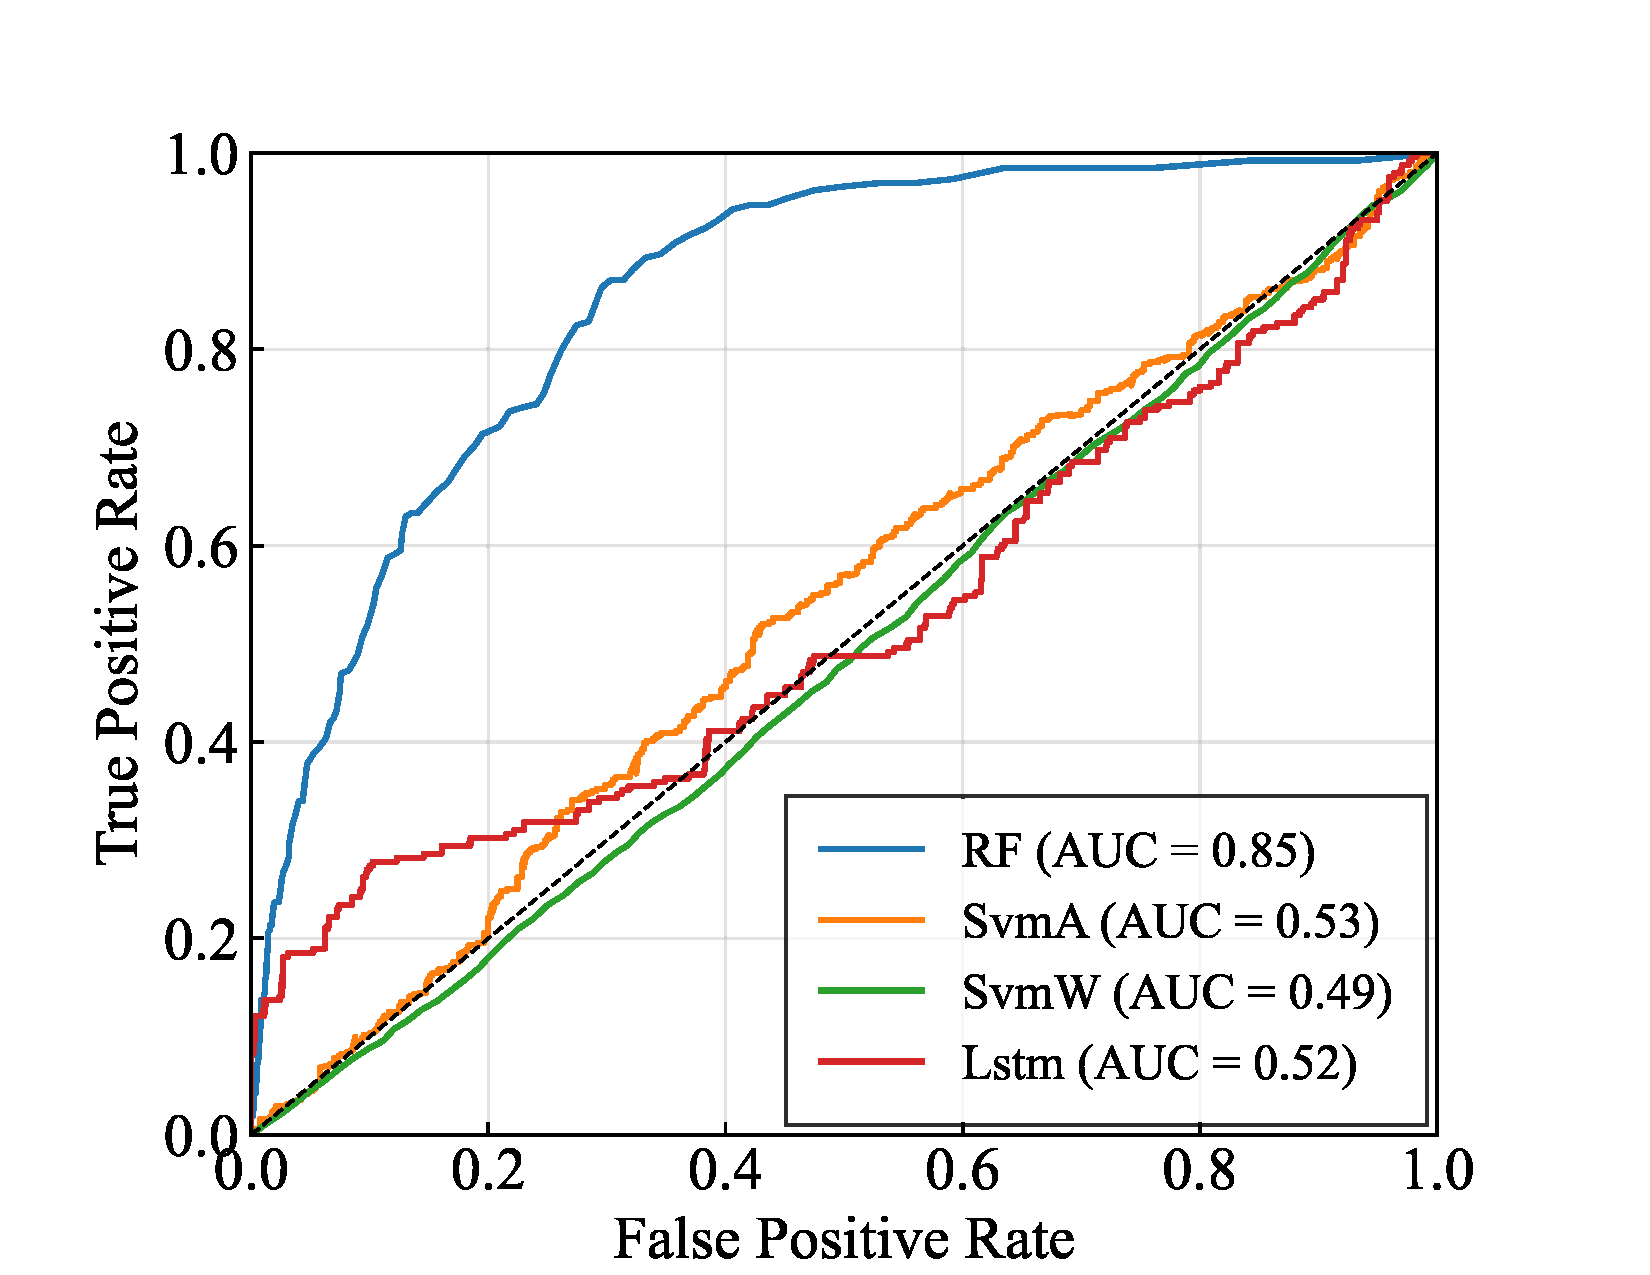
\includegraphics[width=0.5\textwidth]{fig/roc_em.pdf}}
    \caption{ROC curves.}
    \label{roc}
\end{figure} 

\subsection{Discussion}

Overall, we consider that the performance of \Impl{RF} was the highest.
%
\Review{From a qualitative perspective, several factors can explain why \Impl{RF} outperformed the others.}
% 理由１：RFが高い精度を出すことができた主な理由は，他手法よりもの多くの特徴量を用いたから
The primary reason for the high accuracy was that \Impl{RF} model utilized more features than other methods.
%The RF model demonstrated the best performance, possibly because it utilized all available features.%, leading to improved accuracy. 
% 理由２：ArefnezhadとRFの比較を通して，なぜRFが最も良い精度だったかを説明する
\Impl{SvmA}, trained using ANFIS, likely suffered from overfitting, which led to reduced test accuracy. 
In contrast, our proposed RF-based approach effectively avoided overfitting and gained better generalizability. 
% 理由３：ZhaoとRFの比較
As discussed in Sect.~\ref{sec:ddd_svmA}, \Impl{SvmW} used the entire dataset as input, unlike other methods that utilized time windows;
this approach may had led to lower accuracy because long time windows include irrelevant information, which makes it difficult to detect short-term variations. 
By leveraging time-windowed datasets, \Impl{RF} overcame this limitation and maintained higher performance.
% 理由４：WangとRFの比較
\Impl{Lstm} may achieve high accuracy on datasets like those used by Wang et al., where signals exhibit significant changes before and after tasks. 
However, for datasets with minimal signal variation, such as the straight-driving dataset used in this study, the time window may have been too short for \Impl{Lstm} to effectively capture patterns.

\section{\Review{Threats to Validity}}\label{sec:threats}

\subsection{Hyperparameter Optimization}
The hyperparameters of RF, LSTM, and SVM may not have been equally optimized.
RF tends to perform well even with default settings, whereas LSTM and SVM require proper tuning.
If our implementation lacks sufficient optimization, \Impl{SvmA}, \Impl{SvmW} and \Impl{Lstm} may underperform, leading to an unfair evaluation.

\subsection{Feature Bias Towards RF}
The RF model utilizes all the features from other models, which may have given it an advantage.
If the other models used the same full set of features as RF, their performance could potentially improve.

\subsection{Dataset Generalizability}
The dataset used in this study consists of a driving task in a simulator on a straight road at a constant speed. 
While the road shape characteristics play a role, variations in task types could also influence model performance. Since the driving scenario involves minimal steering movements and little acceleration variation, the recorded vehicle dynamics signals may not fully capture real-world driving conditions. 
In more complex scenarios with curved roads or frequent acceleration and deceleration, these signals may behave very differently, potentially limiting the performance of \Impl{RF}.

%\subsubsection{Sample Size}
%LSTM and SVM, in particular, require a large amount of data for effective learning.
%Additionally, Additionally, the class imbalance due to the limited number of abnormal cases may not have been adequately considered.

\subsection{Individual Differences}
Driving behavior and the manifestation of drowsiness in EEG signals may vary among individuals.
Considering these individual differences among subjects may improve model accuracy.
%The timing of drowsiness indicators in EEG and driving behavior may vary between individuals.
%Therefore, using EEG as the ground truth labels and applying the same model to other subjects may not achieve the same level of accuracy.

\section{Conclusion}\label{sec:concl}

This study highlights the importance of reproducibility and standardized development process in the domain of DDD. 
As a result of a reproduction experiment using open data under a common framework, there were several cases where our results differed significantly from the results reported in the original papers.
\Review{In particular, the proposed RF-based method achieved the highest AUC of 0.85 and accuracy of 88\,\% among the four evaluated methods.}
As a bi-product, we have developed a concise RF-based DDD method that uses integrated feature set;
in comparative experiments using standardized performance metrics, it demonstrated the best performance.
%
Future issues include the development of DDD methods using larger-scale ML models, further evaluation experiments after preparing more diverse open datasets, and the deployment in actual vehicles to reduce fatigue-related accidents.
%refining feature selection techniques, incorporating additional data sources, and enhancing real-time detection capabilities.

%\section*{Acknowledgment}



%\section*{References}

\begin{thebibliography}{00}
\bibitem{Milter1988} M. M. Mitler, M. A. Carskadon, C. A. Czeisler, W. C. Dement, D. F. Dinges, and R. C. Graeber, 
    ``Catastrophes, sleep, and public policy: consensus report,'' 
    \textit{Sleep}, vol. 11, no. 1, pp.~100--109, Feb. 1988, DOI: 10.1093/sleep/11.1.100.
\bibitem{Albadawi2022} Y. Albadawi, M. Takruri, and M. Awad,  
    ``A Review of Recent Developments in Driver Drowsiness Detection Systems,''  
    \textit{Sensors}, vol. 22, no. 5, article 2069, 2022, DOI: 10.3390/s22052069.
\bibitem{Perkins2023} E. Perkins, C. Sitaula, M. Burke, and F. Marzbanrad,  
    ``Challenges of Driver Drowsiness Prediction: The Remaining Steps to Implementation,''  
    \textit{IEEE Transactions on Intelligent Vehicles}, vol. 8, no. 2, pp.~1319--1338, Feb. 2023, DOI: 10.1109/TIV.2022.3224690.
\bibitem{Arefnezhad2019} S. Arefnezhad, S. Samiee, A. Eichberger, and A. Nahvi,
    ``Driver Drowsiness Detection Based on Steering Wheel Data Applying Adaptive Neuro-Fuzzy Feature Selection,''
    \textit{Sensors}, vol. 19, no. 4, article 943, 2019, DOI: 10.3390/s19040943.
\bibitem{Zhao2009} S. F. Zhao, G. H. Xu, and T. Fei,
    ``Detecting Driver's Drowsiness Using Multiwavelet Packet Energy Spectrum,''
    \textit{Proceedings of the 2009 International Congress on Image and Signal Processing}, pp.~1--5, 2009, DOI: 10.1109/CISP.2009.5301253.
\bibitem{Wang2022} X. Wang, R. Xu, S. Zhang, Y. Zhuang, and Y. Wang,
    ``Driver Distraction Detection Based on Vehicle Dynamics Using Naturalistic Driving Data,''
    \textit{Transportation Research Part C: Emerging Technologies}, vol. 136, article 103561, 2022, DOI: 10.1016/j.trc.2022.103561.
\bibitem{Kapoor2023} S. Kapoor, and A. Narayanan. 
    ``Leakage and the Reproducibility Crisis in Machine-Learning-Based Science.''
    \textit{Patterns}, vol. 4, no. 9, article 100804, Sep. 2023, DOI: 10.1016/j.patter.2023.100804.
%\bibitem{Romera2016} E. Romera, L. M. Bergasa, and R. Arroyo,  
%    ``Need Data for Driving Behavior Analysis? Presenting the Public UAH-DriveSet,''  
%    in \textit{Proc. IEEE Int. Conf. Intell. Transp. Syst. (ITSC)}, Rio de Janeiro, Brazil, Nov. 2016, pp. 387-392.
\bibitem{Li2022} W. Li, G. Guo, R. Tan, Y. Xing, G. Li, S. Li, \textit{et al.},  
    ``PPB-Emo: A Multimodal Psychological, Physiological and Behavioural Dataset for Human Emotions in Driving Tasks,''  
    \textit{figshare}, Collection, 2022, DOI: 10.6084/m9.figshare.c.5744171.v1. 
    %Available: \url{https://doi.org/10.6084/m9.figshare.c.5744171.v1}.
\bibitem{Eichberger2022} A. Eichberger and S. Arefnezhad,  
    ``Dataset `FULL' for Drowsiness Detection in Drivers,'' 
    \textit{Graz University of Technology}, 2022, DOI: 10.3217/8z09d-nrj27. 
    %Available: \url{https://doi.org/10.3217/8z09d-nrj27}.
\bibitem{Arefnezhad2020} S. Arefnezhad, S. Samiee, A. Eichberger, M. Frühwirth, C. Kaufmann, and E. Klotz,  
    ``Applying Deep Neural Networks for Multi-Level Classification of Driver Drowsiness Using Vehicle-Based Measures,''  
    \textit{Expert Systems with Applications}, vol. 162, article 113778, 2020, DOI: 10.1016/j.eswa.2020.113778.
\bibitem{Aygun2024} A. Aygun, G. Blaney, Z. Haga, T. McWilliams, J. Mertens, J. P. de Ruiter, M. Scheutz, and N. Ward, 
    ``Multi-modal Data Acquisition Platform for Behavioral Evaluation,''  
    \textit{Harvard Dataverse}, version 2, 2024, DOI: 10.7910/DVN/HMZ5RG. 
    %Available: \url{https://doi.org/10.7910/DVN/HMZ5RG}.
\bibitem{Xue2023} Q. Xue, X. Wang, Y. Li, and W. Guo,  
    ``Young Novice Drivers’ Cognitive Distraction Detection: Comparing Support Vector Machines and Random Forest Model of Vehicle Control Behavior,''  
    \textit{Sensors}, vol. 23, no. 3, article 1345, Jan. 2023. DOI: 10.3390/s23031345.
%\bibitem{Tango2013} Tango,
%    ``Real-Time Detection System of Driver Distraction Using Machine Learning,''
%    \textit{Proceedings of the 2013 IEEE Intelligent Vehicles Symposium}, vol. 1, pp. 200--206, 2013.
%\bibitem{Jeon2021} Jeon,
%    ``Ensemble CNN to Detect Drowsy Driving with In-Vehicle Sensor Data,''
%    \textit{Proceedings of the 2021 IEEE Intelligent Vehicles Symposium}, vol. 1, pp. 115--120, 2021.
%\bibitem{Barta2012} Barta,
%    ``A feasibility study of drowsiness detection using driving behaviour parameters,''
%    \textit{Proceedings of the 2012 International Conference on Driver Distraction and Inattention}, vol. 1, pp. 101--110, 2012.
\bibitem{Li2017_2} Z. Li, L. Chen, J. Peng, and Y. Wu,  
    ``Automatic Detection of Driver Fatigue Using Driving Operation Information for Transportation Safety,''  
    \textit{Sensors}, vol. 17, no. 6, article~1212, May 2017. DOI: 10.3390/s17061212.
\bibitem{Krajewski2009} J. Krajewski, D. Sommer, U. Trutschel, D. Edwards, and M. Golz,  
    ``Steering Wheel Behavior Based Estimation of Fatigue,''  
    \textit{Proceedings of the Driving Assessment Conference}, pp.~118--124, 2009. DOI: 10.17077/drivingassessment.1311.
\bibitem{Eskandarian2007} A. Eskandarian and A. Mortazavi,  
    ``Evaluation of a Smart Algorithm for Commercial Vehicle Driver Drowsiness Detection,''  
    \textit{Proceedings of the 2007 IEEE Intelligent Vehicles Symposium}, Istanbul, Turkey, pp.~553--559, 2007. DOI: 10.1109/IVS.2007.4290173.
\bibitem{Mcdonald2014} A. D. McDonald, J. D. Lee, C. Schwarz, and T. L. Brown,  
    ``Steering in a Random Forest: Ensemble Learning for Detecting Drowsiness-Related Lane Departures,''  
    \textit{Human Factors}, vol. 56, no. 5, pp.~986--998, 2014. DOI: 10.1177/0018720813515272.
\bibitem{Mcdonald2012} A. McDonald, C. Schwarz, J. Lee, and T. Brown,  
    ``Real-Time Detection of Drowsiness Related Lane Departures Using Steering Wheel Angle,''  
    \textit{Proceedings of the Human Factors and Ergonomics Society Annual Meeting}, vol. 56, pp.~210--215, 2012. %DOI: 10.1177/1071181312561464.
\bibitem{Li2017} Z. Li, S. E. Li, R. Li, B. Cheng, and J. Shi,  
    ``Online Detection of Driver Fatigue Using Steering Wheel Angles for Real Driving Conditions,''  
    \textit{Sensors}, vol. 17, no. 3, article 495, Mar. 2017. DOI: 10.3390/s17030495.
\bibitem{Sandberg2008} D. Sandberg and M. Wahde,  
    ``Particle Swarm Optimization of Feedforward Neural Networks for the Detection of Drowsy Driving,''  
    \textit{Proceedings of the 2008 IEEE International Joint Conference on Neural Networks (IEEE World Congress on Computational Intelligence)}, Hong Kong, China, pp.~788--793, 2008. DOI: 10.1109/IJCNN.2008.4633886.
\bibitem{Chai2019} M. Chai, S. Li, W. Sun, M. Guo, and M. Huang,  
    ``Drowsiness Monitoring Based on Steering Wheel Status,''  
    \textit{Transportation Research Part D: Transport and Environment}, vol. 66, pp.~95--103, 2019. DOI: 10.1016/j.trd.2018.07.007.
\bibitem{Jin2012} L. Jin, Q. Niu, H. Hou, H. Xian, Y. Wang, and D. Shi,  
    ``Driver Cognitive Distraction Detection Using Driving Performance Measures,''  
    \textit{Discrete Dynamics in Nature and Society}, vol. 2012, Art. no. 432634, Nov. 2012. DOI: 10.1155/2012/432634.
\bibitem{Jung1997} T. P. Jung, S. Makeig, M. Stensmo, and T. J. Sejnowski,  
    ``Estimating alertness from the EEG power spectrum,''  
    \textit{IEEE Transactions on Biomedical Engineering}, vol. 44, no. 1, pp.~60--69, Jan. 1997. DOI: 10.1109/10.553713.
\bibitem{Horne2004} J. A. Horne and S. D. Baulk,  
    ``Awareness of sleepiness when driving,''  
    \textit{Psychophysiology}, vol. 41, no. 1, pp.~161--165, Jan. 2004. DOI: 10.1046/j.1469-8986.2003.00130.x.
\bibitem{Jap2009} B. Jap, S. Budi, S. Lal, P. Fischer, and E. Bekiaris,  
    ``Using EEG spectral components to assess algorithms for detecting fatigue [Part 1],''  
    \textit{Expert Systems with Applications}, vol. 36, pp.~2352-2359, 2009. DOI: 10.1016/j.eswa.2007.12.043.
\bibitem{Scheutz2024} M. Scheutz, S. Aeron, A. Aygun, J. P. de Ruiter, S. Fantini, C. Fernandez, Z. Haga, T. Nguyen, and B. Lyu,  
    ``Estimating Systemic Cognitive States from a Mixture of Physiological and Brain Signals,''  
    \textit{Topics in Cognitive Science}, vol. 16, no. 3, pp.~485--526, Jul. 2024. DOI: 10.1111/tops.12669.
\bibitem{Breiman2001} L. Breiman,  
    ``Random Forests,''
    \textit{Machine Learning}, vol.~45, no.~1, pp.~5--32, Oct. 2001. DOI: 10.1023/A:1010933404324.

% \bibitem{McDonald2014} McDonald,
%     ``Steering in a Random Forest: Ensemble Learning for Detecting Drowsiness-Related Lane Departures,''
%    ｋ  \textit{Proceedings of the 2014 IEEE Intelligent Vehicles Symposium}, vol. 1, pp. 234--241, 2014.
% \bibitem{Zhang2016} Zhang,
%     ``Sensitivity of Lane Position and Steering Angle Measurements to Driver Fatigue,''
%     \textit{Proceedings of the 2016 IEEE Intelligent Vehicles Symposium}, vol. 1, pp. 456--463, 2016.
%    \bibitem{he2009} H. He and E. A. Garcia, 
%    ``Learning from Imbalanced Data,'' 
%    \textit{IEEE Transactions on Knowledge and Data Engineering}, vol. 21, no. 9, pp.~1263--1284, Sept. 2009, doi: 10.1109/TKDE.2008.239.
%    \bibitem{Breiman2001} L. Breiman, ``Random Forests,''
%    \textit{Machine Learning}, vol. 45, no. 1, pp.~5--32, 2001. 
%    DOI: \url{https://doi.org/10.1023/A:1010933404324}
\end{thebibliography}

\end{document}
